% This file was created by tikzplotlib v0.9.3.
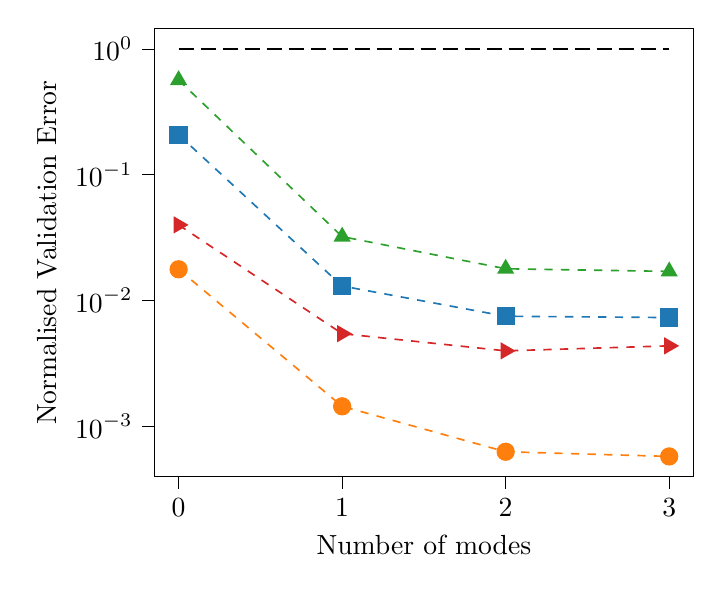
\begin{tikzpicture}

\definecolor{color0}{rgb}{0.12156862745098,0.466666666666667,0.705882352941177}
\definecolor{color1}{rgb}{1,0.498039215686275,0.0549019607843137}
\definecolor{color2}{rgb}{0.172549019607843,0.627450980392157,0.172549019607843}
\definecolor{color3}{rgb}{0.83921568627451,0.152941176470588,0.156862745098039}

\begin{axis}[
log basis y={10},
tick align=outside,
tick pos=left,
x grid style={white!69.0196078431373!black},
xlabel={Number of modes},
xmin=-0.15, xmax=3.15,
xtick style={color=black},
xtick={0,1,2,3},
xticklabels={\(\displaystyle 0\),\(\displaystyle 1\),\(\displaystyle 2\),\(\displaystyle 3\)},
y grid style={white!69.0196078431373!black},
ylabel={Normalised Validation Error},
ymin=0.000396112842703244, ymax=1.45214044883202,
ymode=log,
ytick style={color=black},
ytick={1e-05,0.0001,0.001,0.01,0.1,1,10,100},
yticklabels={\(\displaystyle 10^{-5}\),\(\displaystyle 10^{-4}\),\(\displaystyle 10^{-3}\),\(\displaystyle 10^{-2}\),\(\displaystyle 10^{-1}\),\(\displaystyle 10^{0}\),\(\displaystyle 10^{1}\),\(\displaystyle 10^{2}\)}
]
\path [draw=black, semithick, dash pattern=on 5.55pt off 2.4pt]
(axis cs:0,1)
--(axis cs:3,1);

\addplot [semithick, color0, dashed, mark=square*, mark size=3, mark options={solid}]
table {%
0 0.207379162311554
1 0.0130139421671629
2 0.00748647097498178
3 0.00731012364849448
};
\addplot [semithick, color1, dashed, mark=*, mark size=3, mark options={solid}]
table {%
0 0.0176829695701599
1 0.00143955205567181
2 0.000626487308181822
3 0.000575211481191218
};
\addplot [semithick, color2, dashed, mark=triangle*, mark size=3, mark options={solid}]
table {%
0 0.564595460891724
1 0.0321590229868889
2 0.0178603641688824
3 0.0170018896460533
};
\addplot [semithick, color3, dashed, mark=triangle*, mark size=3, mark options={solid,rotate=270}]
table {%
0 0.0398590378463268
1 0.00544324843212962
2 0.00397256063297391
3 0.00435326993465424
};
\end{axis}

\end{tikzpicture}
